\documentclass[12pt, a4paper]{article}

% --- Core Packages ---
\usepackage[utf8]{inputenc}
\usepackage{geometry}
\geometry{a4paper, margin=2.5cm}
\usepackage{graphicx}
\usepackage{float}
\usepackage{hyperref}
\usepackage{amsmath}

\graphicspath{{../results/project/plots/}}

% --- Document Information ---
\title{Machine Learning and Pattern Recognition\\ \large Laboratory 04: Probability and Density Estimation}
\author{Nicola Beccaceci}
\date{}

\begin{document}

\maketitle

\section*{1D Gaussian Density Estimation}

In this laboratory, we investigate the underlying distributions of the dataset features for both the Fake (label 0) and Genuine (label 1) classes. To do so, we fit uni-variate Gaussian models to the empirical data using Maximum Likelihood Estimation (MLE). By plotting the continuous Gaussian probability density function (PDF) curves on top of the normalized discrete empirical histograms, we can visually and theoretically evaluate the validity of the normal distribution assumption for each specific feature within our dataset.

\subsection*{Question 1: What do you observe?}

\subsubsection*{Empirical Results}
Upon visual inspection of the density plots, we observe a distinct dichotomy in the geometric structure of the dataset's distributions. The majority of the features, specifically Features 1 through 4, present a standard, unimodal geometry for both the Fake and Genuine classes. These features are generally symmetric and possess a single, central peak. However, Features 5 and 6 exhibit significantly more complex topological structures, breaking the standard normality assumption. Most notably, the Genuine class for Features 5 and 6 displays clearly bimodal distributions, characterized by two distinct peaks separated by an area of low sample density (a "valley"). The Fake class for these features, while unimodal, exhibits heavier tails and slight skewness compared to a perfect Gaussian curve.

\subsubsection*{Theoretical Analysis}
The Gaussian assumption relies on the probability density function defined as:
\[
\mathcal{N}(x | \mu, \sigma^2) = \frac{1}{\sqrt{2\pi\sigma^2}} \exp\left( -\frac{(x - \mu)^2}{2\sigma^2} \right)
\]
To fit this model, the Maximum Likelihood Estimator (MLE) computes the sample mean ($\mu_{ML}$) and sample variance ($\sigma^2_{ML}$) that maximize the log-likelihood of observing the training data. For unimodal distributions (Features 1-4), this optimization successfully centers the continuous density over the data's empirical center of mass, and the variance accurately captures the data's spread. 

However, for multi-modal geometries (Features 5-6), a single Gaussian distribution lacks the necessary degrees of freedom (capacity) to accurately describe the data. The MLE, forced to find a single optimal mean, compromises by placing the mean $\mu_{ML}$ directly between the multiple modes. Consequently, the single variance parameter $\sigma^2_{ML}$ is artificially inflated to encompass both peaks. This results in a severe mismatch between the theoretical model and the empirical reality, as the model predicts the highest probability density in regions where the actual sample count is minimal.

\subsection*{Question 2: Are there features for which the Gaussian densities provide a good fit?}

Yes, the 1D Gaussian model provides a highly accurate fit for \textbf{Features 1, 2, 3, and 4} across both the Fake and Genuine classes.

\subsubsection*{Detailed Feature Analysis}

\begin{figure}[H]
    \centering
    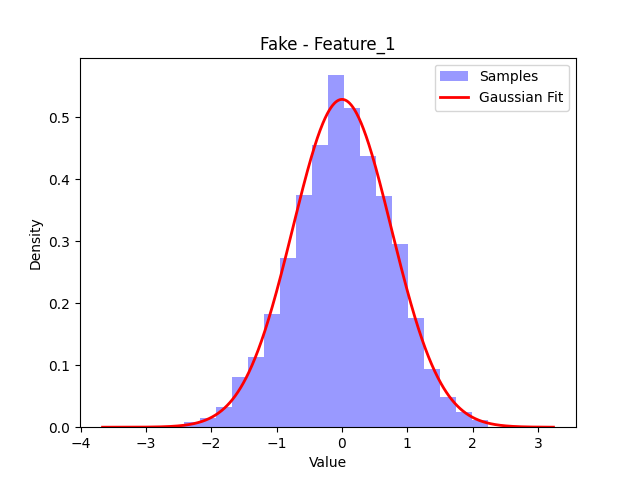
\includegraphics[width=0.48\linewidth]{fake_feature_1.png}
    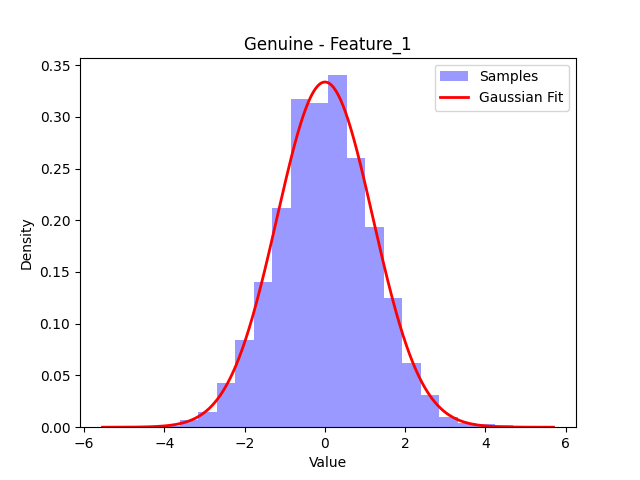
\includegraphics[width=0.48\linewidth]{genuine_feature_1.png}
    \caption{Gaussian fit for Feature 1. Fake class (left) and Genuine class (right).}
    \label{fig:feature_1}
\end{figure}
\textbf{Feature 1:} The empirical histograms are highly symmetric and unimodal. The estimated Gaussian curves wrap the data perfectly. The Maximum Likelihood estimators for the mean and variance effectively capture the central tendency and dispersion of the data without systematic bias.

\begin{figure}[H]
    \centering
    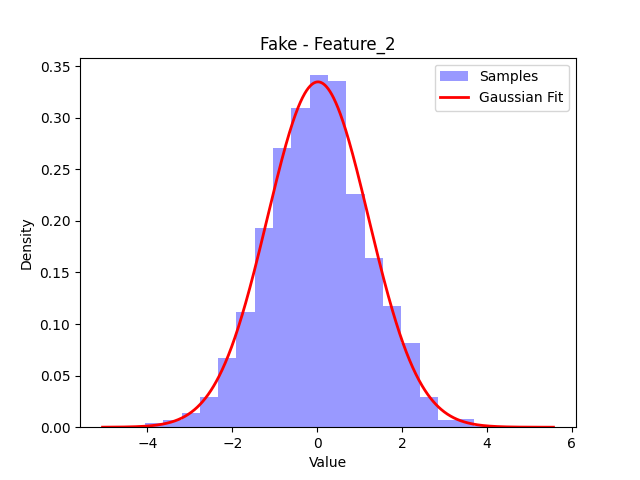
\includegraphics[width=0.48\linewidth]{fake_feature_2.png}
    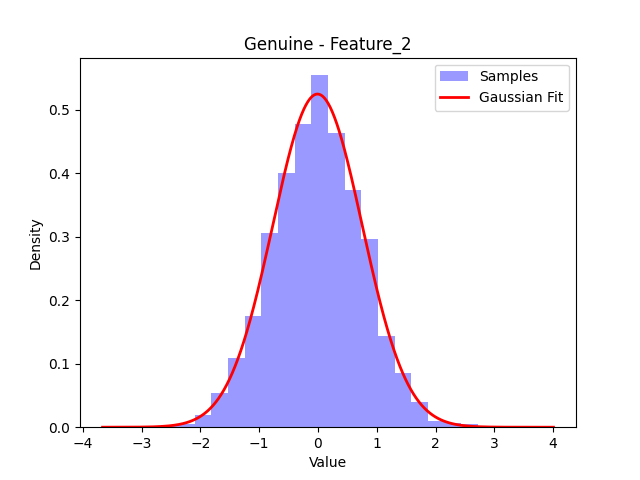
\includegraphics[width=0.48\linewidth]{genuine_feature_2.png}
    \caption{Gaussian fit for Feature 2. Fake class (left) and Genuine class (right).}
    \label{fig:feature_2}
\end{figure}
\textbf{Feature 2:} Similar to Feature 1, the distributions here follow a strong normal pattern. Both classes exhibit a prominent central peak, and the exponential decay in the tails strictly adheres to the Gaussian PDF formula.

\begin{figure}[H]
    \centering
    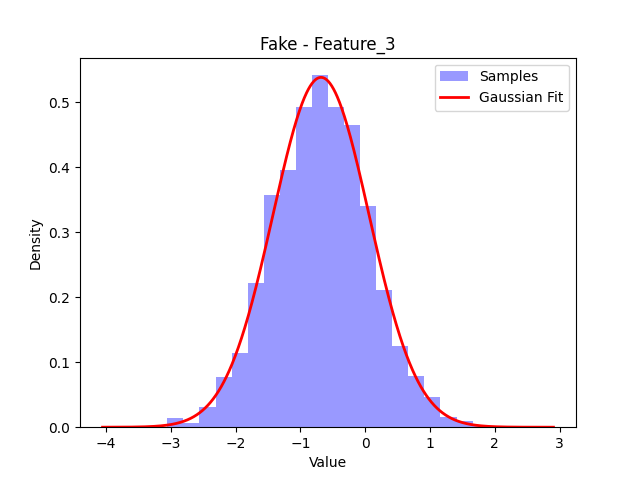
\includegraphics[width=0.48\linewidth]{fake_feature_3.png}
    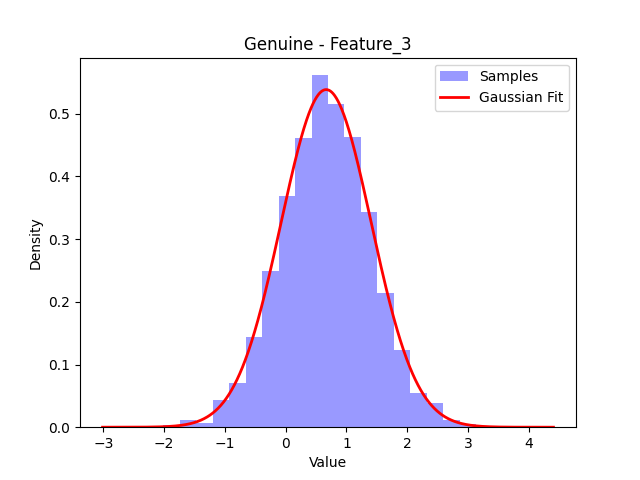
\includegraphics[width=0.48\linewidth]{genuine_feature_3.png}
    \caption{Gaussian fit for Feature 3. Fake class (left) and Genuine class (right).}
    \label{fig:feature_3}
\end{figure}
\textbf{Feature 3:} The Genuine class shows a particularly excellent fit, where the empirical frequencies at almost every bin align with the theoretical curve. The Fake class shows minor noise but mathematically remains well-represented by the Gaussian distribution.

\begin{figure}[H]
    \centering
    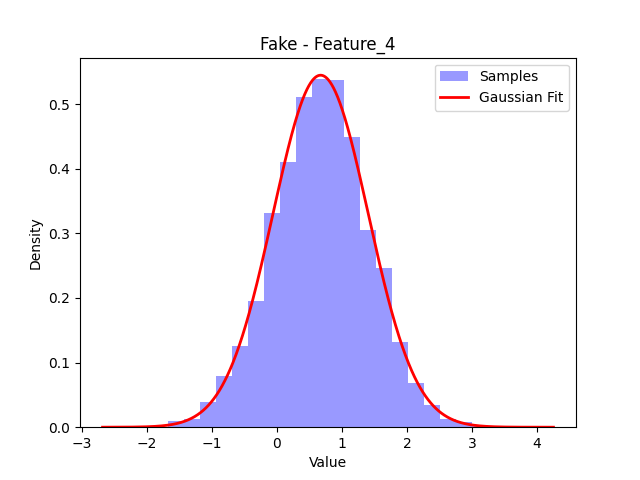
\includegraphics[width=0.48\linewidth]{fake_feature_4.png}
    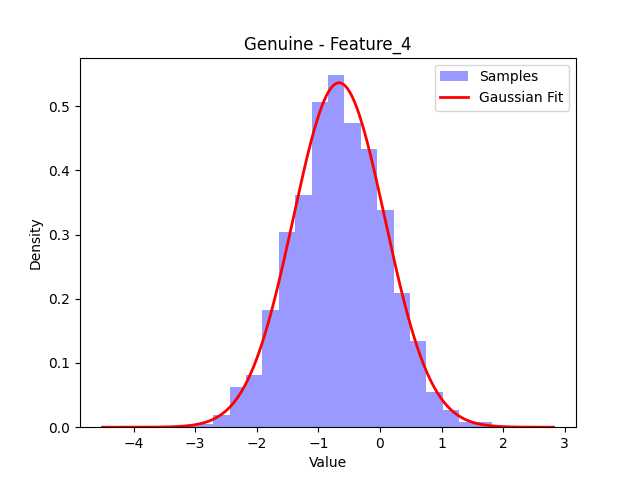
\includegraphics[width=0.48\linewidth]{genuine_feature_4.png}
    \caption{Gaussian fit for Feature 4. Fake class (left) and Genuine class (right).}
    \label{fig:feature_4}
\end{figure}
\textbf{Feature 4:} The underlying data generation process for this feature mimics a normal distribution closely. The lack of heavy skewness means that the two parameters ($\mu$ and $\sigma^2$) contain sufficient mathematical capacity to fully describe the class-conditional densities.


\subsection*{Question 3: Are there features for which the Gaussian model seems significantly less accurate?}

Yes, the Gaussian model is significantly inaccurate for \textbf{Features 5 and 6}, particularly due to the complex topology of the Genuine class.

\subsubsection*{Detailed Feature Analysis}

\begin{figure}[H]
    \centering
    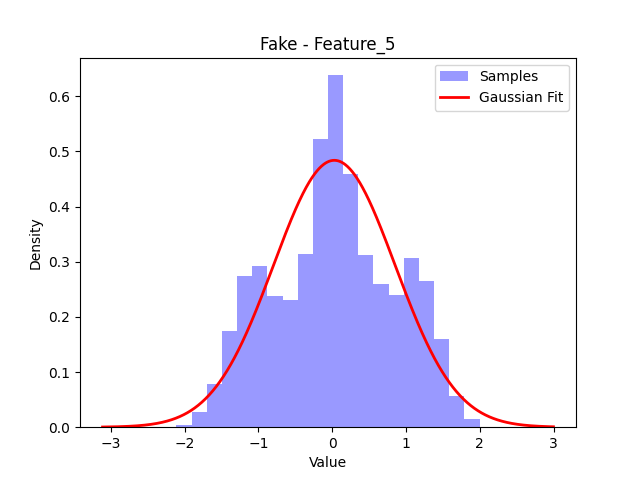
\includegraphics[width=0.48\linewidth]{fake_feature_5.png}
    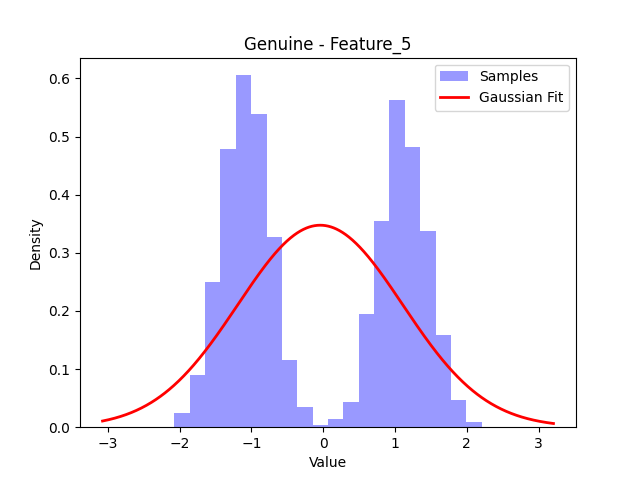
\includegraphics[width=0.48\linewidth]{genuine_feature_5.png}
    \caption{Gaussian fit for Feature 5. Fake class (left) and Genuine class (right). Note the bimodal nature of the Genuine class.}
    \label{fig:feature_5}
\end{figure}
\textbf{Feature 5:} The Genuine class is strictly \textbf{bimodal}. The empirical data is split into two distinct, high-density peaks separated by a wide, empty "valley." The Gaussian distribution, being mathematically constrained to be unimodal and symmetric, is fundamentally incompatible with this geometry. When applying MLE, the model calculates the global mean, placing the absolute highest probability peak of the bell curve directly at the center coordinates—exactly inside the empty valley where almost zero empirical samples exist. 

\begin{figure}[H]
    \centering
    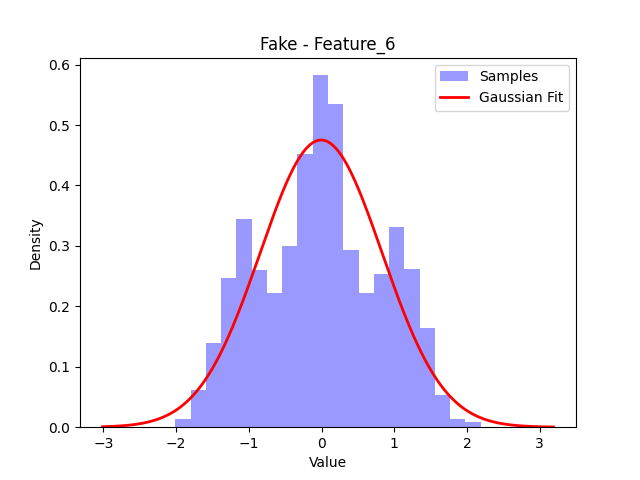
\includegraphics[width=0.48\linewidth]{fake_feature_6.png}
    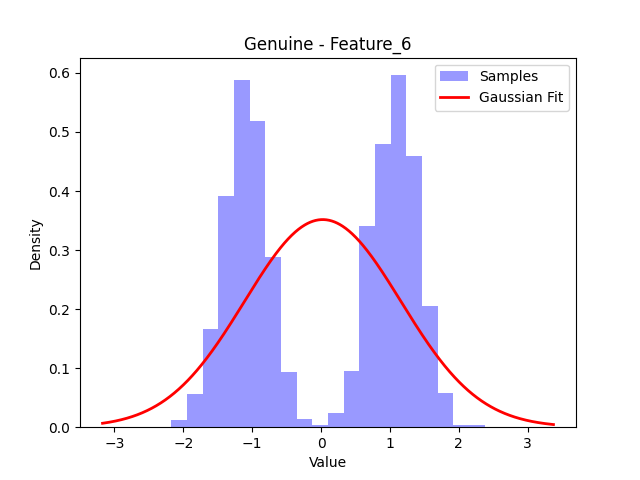
\includegraphics[width=0.48\linewidth]{genuine_feature_6.png}
    \caption{Gaussian fit for Feature 6. Fake class (left) and Genuine class (right). The Gaussian model heavily underestimates the dual peaks of the Genuine class.}
    \label{fig:feature_6}
\end{figure}
\textbf{Feature 6:} Similarly, the Genuine class exhibits strong bimodality. The estimated Gaussian curve flattens out, attempting to cover both peaks, thereby drastically underestimating the density at the actual modes and overestimating it in the center. Furthermore, in the Fake class, while technically unimodal, the feature exhibits heavier tails than a standard normal distribution. The rigid shape of the Gaussian bell curve fails to capture these extended tails accurately.

\subsection*{Implications for Future Laboratories and Model Selection}

This visual and theoretical proof of non-normality in Features 5 and 6 is critical for the architectural design of our classification system in subsequent laboratories. The failure of the uni-variate Gaussian to model these features has direct consequences for multivariate generative models.

\begin{enumerate}
    \item \textbf{Failure of Simple Generative Models:} If we deploy a Naive Bayes classifier or a generative classifier based on a single Multivariate Gaussian (such as the standard MVG or Tied MVG), the model will intrinsically assume unimodality. For a test sample belonging to the Genuine class that falls into one of the two actual peaks of Features 5 or 6, the single-Gaussian model will assign it a relatively low likelihood. Conversely, it will assign high log-likelihoods to theoretical test samples falling in the empty center, guaranteeing poor density estimation and directly leading to elevated misclassification rates.
    \item \textbf{Necessity of Gaussian Mixture Models (GMM):} This geometrically proves why our dataset mathematically necessitates the use of more expressive generative models. A Gaussian Mixture Model (GMM), which defines the density as a linear combination of multiple Gaussian components, would be perfectly suited to wrap the multiple localized clusters observed in Features 5 and 6 simultaneously.
    \item \textbf{Transition to Discriminative Models:} Alternatively, this highlights the potential superiority of discriminative models for this specific dataset. Models like Logistic Regression or non-linear Support Vector Machines (SVMs with RBF kernels) do not attempt to model the underlying probability density $P(X|Y)$ but rather focus directly on finding the optimal decision boundary $P(Y|X)$. By projecting the data into higher-dimensional spaces (e.g., using kernels), they can easily separate bimodal distributions without being constrained by parametric density assumptions.
\end{enumerate}

\end{document}